\documentclass{article}
\usepackage[margin=1in]{geometry}
\usepackage{amsmath}
\usepackage{graphicx}
\usepackage{siunitx}
\usepackage{listings}
\usepackage{xcolor}
\usepackage{booktabs}
\usepackage{hyperref}
\definecolor{mygreen}{rgb}{0,0.6,0}
\definecolor{mygray}{rgb}{0.5,0.5,0.5}
\definecolor{mymauve}{rgb}{0.58,0,0.82}

\lstset{ %
  backgroundcolor=\color{white},   % choose the background color; you must add \usepackage{color} or \usepackage{xcolor}
  basicstyle=\scriptsize\ttfamily,    % the size of the fonts that are used for the code
  breakatwhitespace=false,         % sets if automatic breaks should only happen at whitespace
  breaklines=true,                 % sets automatic line breaking
  captionpos=b,                    % sets the caption-position to bottom
  commentstyle=\color{mygreen},    % comment style
  deletekeywords={},            % if you want to delete keywords from the given language
  escapeinside={\%*}{*)},          % if you want to add LaTeX within your code
  extendedchars=true,              % lets you use non-ASCII characters; for 8-bits encodings only, does not work with UTF-8
  frame=shadowbox,                    % adds a frame around the code
%  framexleftmarign=5mm,
  xleftmargin=10pt,
  xrightmargin=10pt,
  rulesepcolor=\color{gray},
  keywordstyle=\color{blue},       % keyword style
  language=Octave,                 % the language of the code
  morekeywords={*,...,fit,predint,export\_fig},            % if you want to add more keywords to the set
%  numbers=left,                    % where to put the line-numbers; possible values are (none, left, right)
  numbers=none,
  numbersep=5pt,                   % how far the line-numbers are from the code
  numberstyle=\tiny\color{mygray}, % the style that is used for the line-numbers
  rulecolor=\color{black},         % if not set, the frame-color may be changed on line-breaks within not-black text (e.g. comments (green here))
  showspaces=false,                % show spaces everywhere adding particular underscores; it overrides 'showstringspaces'
  showstringspaces=false,          % underline spaces within strings only
  showtabs=false,                  % show tabs within strings adding particular underscores
  stepnumber=1,                    % the step between two line-numbers. If it's 1, each line will be numbered
  stringstyle=\color{mymauve},     % string literal style
  tabsize=4,                       % sets default tabsize to 4 spaces
  caption=\lstname                   % show the filename of files included with \lstinputlisting; also try caption instead of title
}


\title{1.723 Final}
\author{Sachith  Dunatunga}

\begin{document}
\newcommand{\deriv}[2]{\frac{\partial #1}{ \partial #2}}
\newcommand{\nderiv}[3]{\frac{\partial^{#3} #1}{ \partial #2^{#3}}}
\newcommand{\dx}[1]{\deriv{#1}{x}}
\newcommand{\taylorexpf}[3]{#1_{#2} + \left(#3 \right) \dx{#1}\biggr\rvert_{#2} + \frac{1}{2}\left(#3 \right)^2 \nderiv{#1}{x}{2}\biggr\rvert_{#2} + \frac{1}{6}\left(#3 \right)^3\nderiv{#1}{x}{3}\biggr\rvert_{#2} + \frac{1}{24}\left(#3 \right)^4\nderiv{#1}{x}{4}\biggr\rvert_{#2} + O(h^5)}
\maketitle

\section{Problem 1}
\subsection{Part 1}
Since we know $\nabla^2 \Psi = - \omega$, we can write
\begin{align}
    \nabla^2 (\Psi_0 + \tilde{\Psi}) &= -\omega \\
    \nabla^2 \Psi_0 + \nabla^2 \tilde{\Psi} &= -\omega.
\end{align}
However, we know that for this problem $\Psi_0 = y$, since $\mathbf{u}_0 = (1, 0)$.
Therefore, the relationship is given by
\begin{align}
    \nabla^2 y + \nabla^2 \tilde{\Psi} &= -\omega \\
    \nabla^2 \tilde{\Psi} &= -\omega.
\end{align}

In Fourier space, derivatives are taken by multiplying by the wavenumber times the imaginary unit.
Thus, if the fourier transform of $\tilde{\Psi}$ is written as $\hat{\tilde{\Psi}}$, the fourier transform of $\nabla^2 \tilde{\Psi}$ is given by
\begin{align}
    \nabla^2 \tilde{\Psi} &= \nderiv{\tilde{\Psi}}{x}{2} + \nderiv{\tilde{\Psi}}{y}{2} \\
\implies \widehat{\nabla^2 \tilde{\Psi}} &= (ik_x)^2 \hat{\tilde{\Psi}} + (ik_y)^2 \hat{\tilde{\Psi}}\\
    \widehat{\nabla^2 \tilde{\Psi}} &= -(k^2_x + k^2_y) \hat{\tilde{\Psi}}.
\end{align}

Since at zero frequency in both x and y we have $\exp(0) = 1$, the fourier transform turns into the average value of the signal.
In this case, since we only care about derivatives of the stream function $\Psi$, this constant is `free' and will not affect the results.

\subsection{Part 2}
From the previous problem we have
\begin{align}
    \widehat{\nabla^2 \tilde{\Psi}} &= -(k^2_x + k^2_y) \hat{\tilde{\Psi}}.
\end{align}
We can write the fourier transform of the equation
\begin{align}
    \nabla^2 \tilde{\Psi} &= -\omega
\end{align}
as
\begin{align}
    -(k^2_x + k^2_y) \hat{\tilde{\Psi}} &= -\hat{\omega} \\
\implies \hat{\tilde{\Psi}} &= \frac{\hat{\omega}}{k^2_x + k^2_y}.
\end{align}
This means that if we consider an explicit scheme, we can write
\begin{align}
\hat{\tilde{\Psi}}^n &= \frac{\hat{\omega}^{n-1}}{k^2_x + k^2_y}
\end{align}
where
\begin{align}
\omega^{n-1} = R \left( \deriv{c}{x}^{n} u_y^{n-1} - \deriv{c}{y}^{n} u_x^{n-1} \right).
\end{align}
We can obtain the necessary derivatives through $\deriv{c}{x} = i k_x \hat{c}$ and $\deriv{c}{y} i k_y \hat{c}$, where $\hat{c}$ is the fourier transform of the current concentration.
We can apply the inverse FFT to this quantity, and then multiply by the velocities from the previous time step.
We then obtain $\hat{\omega}^{n-1}$ by simply applying the FFT to the resultant.
Note that in both cases we apply the 2D FFT.
Although we need to divide by $(k^2_x + k^2_y) = 0$, in this case since it only affects the mean value of $\Psi$ we can arbitrarily set this term to a nonzero constant.
This is because the mean value of the stream function is not important, only its derivatives, which are still accurate.

\subsection{Part 3}
Please see the listing \ref{code:solve-vel} in the appendix for the MATLAB code.
An optimized version of this function, shown in listing \ref{code:solve-vel-opt}, is used for the time stepping (e.g. we generate the wavenumber matrices outside the time loop).
The zip file included also contains the code.

\subsection{Part 4}
Please see the listing \ref{code:solve-conc} in the appendix for the MATLAB code.
An optimized version of this function, shown in listing \ref{code:solve-conc-opt}, is used for the time stepping (e.g. we generate the wavenumber matrices outside the time loop).
The zip file included also contains the code.

\subsection{Part 5}
\begin{enumerate}
\item For the concentration field, the most obvious feature we notice is the development of fingers in the flow.
The initial concentration is show in figure \ref{fig:initial-conc}.
Various snapshots in time are shown in figure \ref{fig:conc} (the final configuration at $t \approx 4$ is shown in figure \ref{fig:final-conc}).
The initially (nearly) vertical ``interface'' (the two fluids are perfectly miscible, so there is no surface tension) quickly disappears.
It looks the mixing should be enhanced by this, as the gradient is sharper along the boundary of the fingers and the arclength is longer as well.
We also see that with higher viscosity contrasts, it looks as though the mixing proceeds faster.
We can confirm this by looking at the variance of concentration and $\epsilon_c$ later.

\begin{figure}[!ht]
\centering
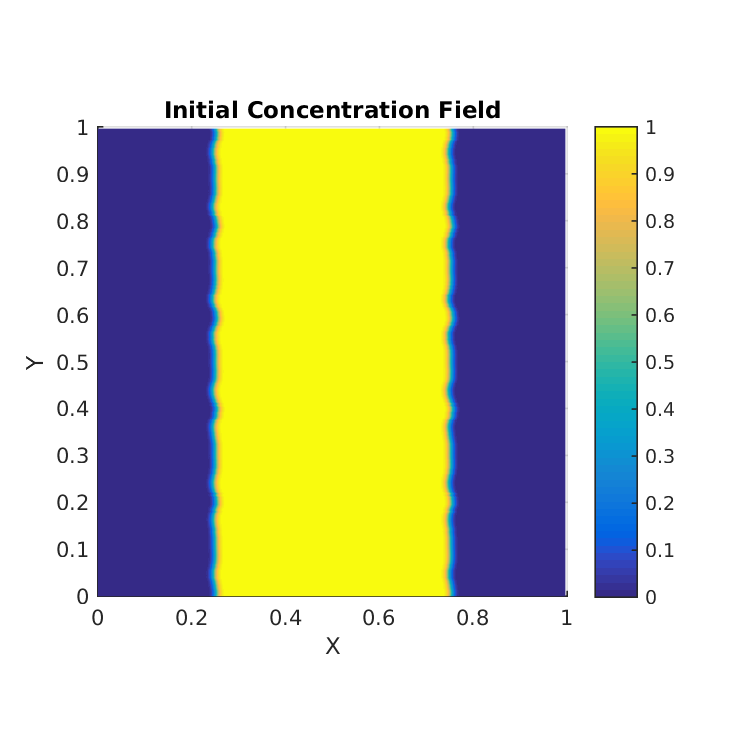
\includegraphics[scale=1.0]{initial_conc.png}
\caption{The initial concentration used for all simulations. There are small pertubations to the otherwise vertical boundary in concentration.}
\label{fig:initial-conc}
\end{figure}

\begin{figure}[!ht]
\centering
\begin{tabular}{c c c}
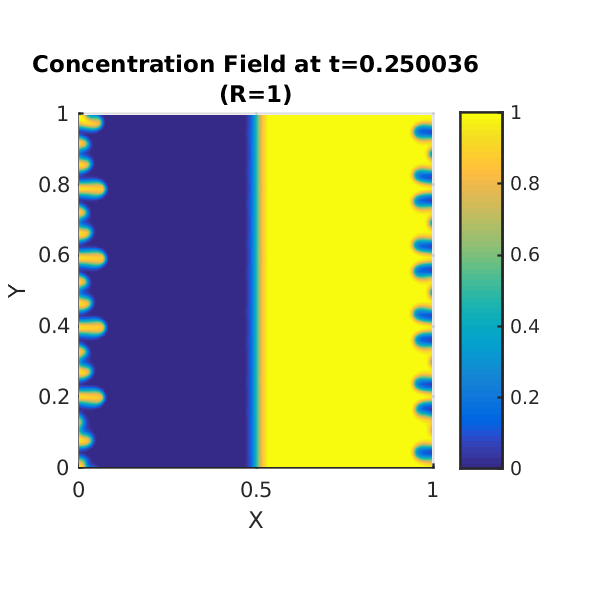
\includegraphics[scale=0.5]{conc10_25.png} &
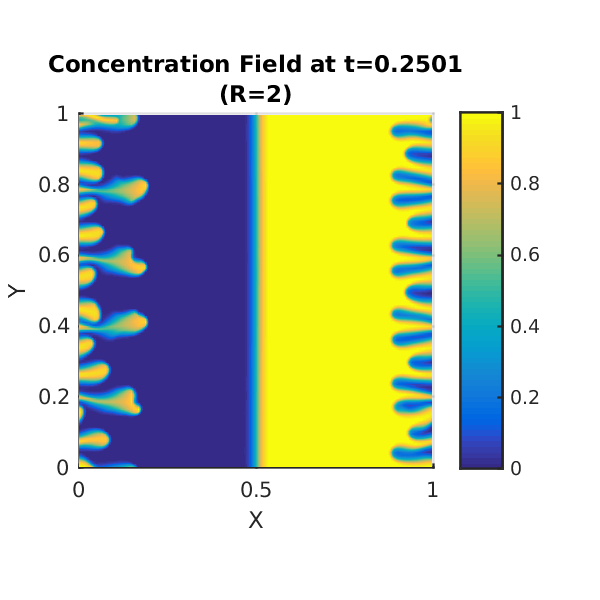
\includegraphics[scale=0.5]{conc20_25.png} &
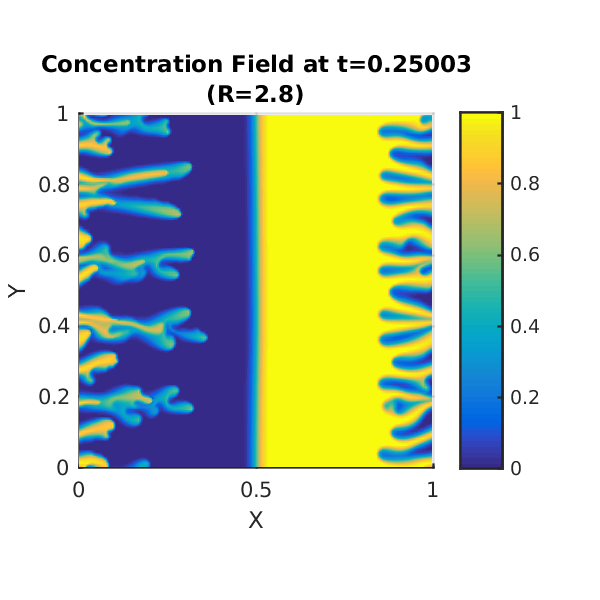
\includegraphics[scale=0.5]{conc28_25.png} \\
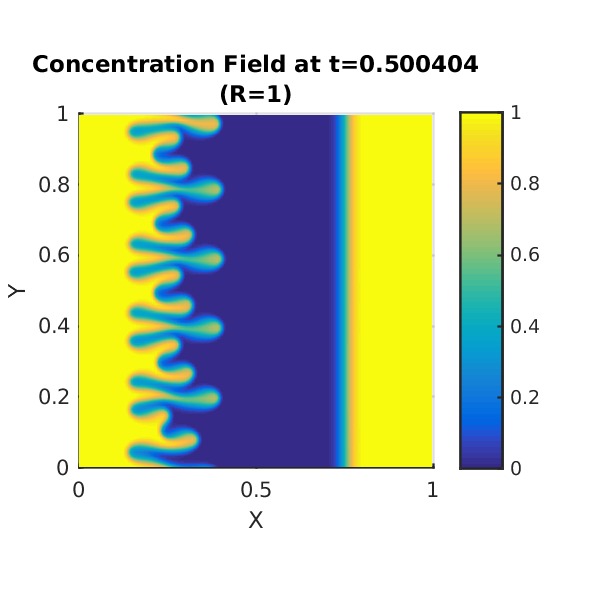
\includegraphics[scale=0.5]{conc10_50.png} &
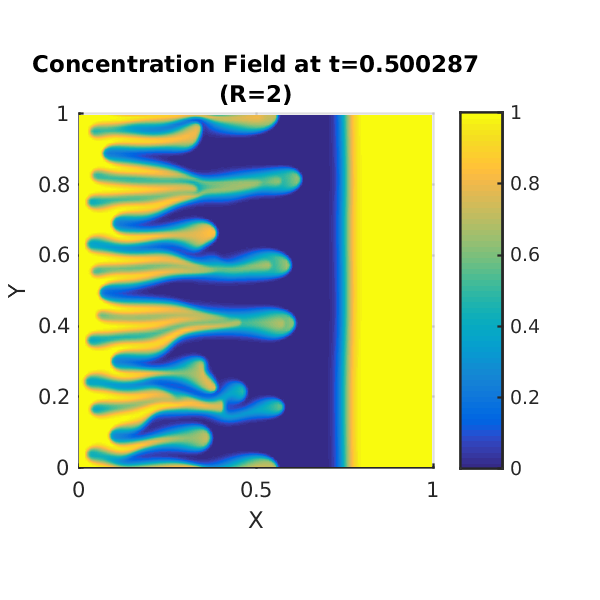
\includegraphics[scale=0.5]{conc20_50.png} &
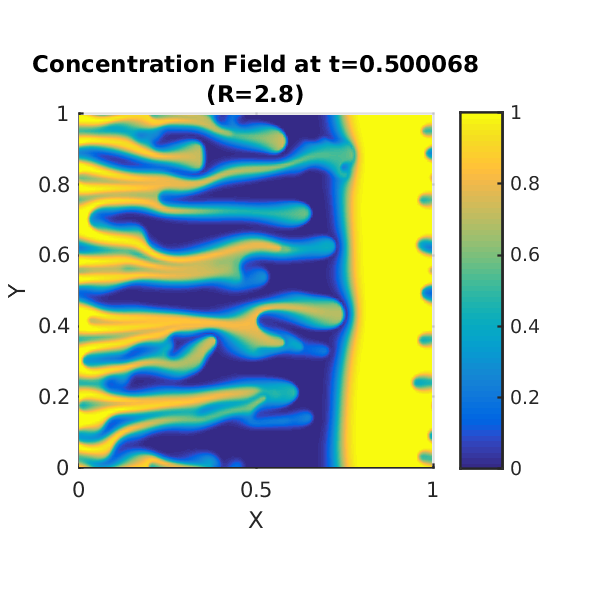
\includegraphics[scale=0.5]{conc28_50.png} \\
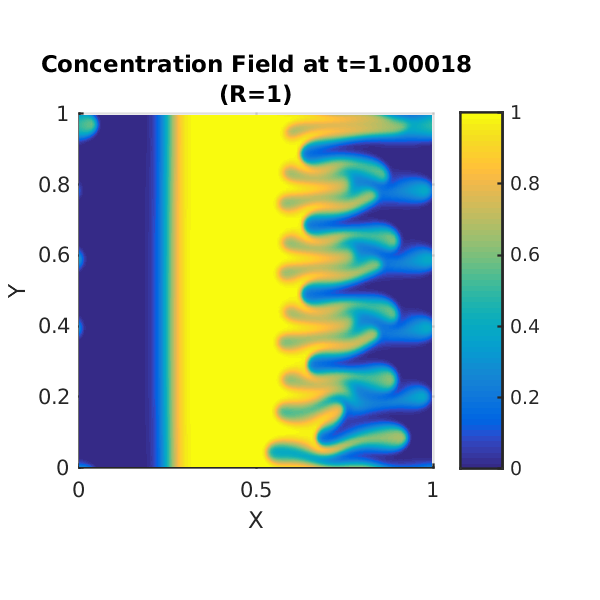
\includegraphics[scale=0.5]{conc10_100.png} &
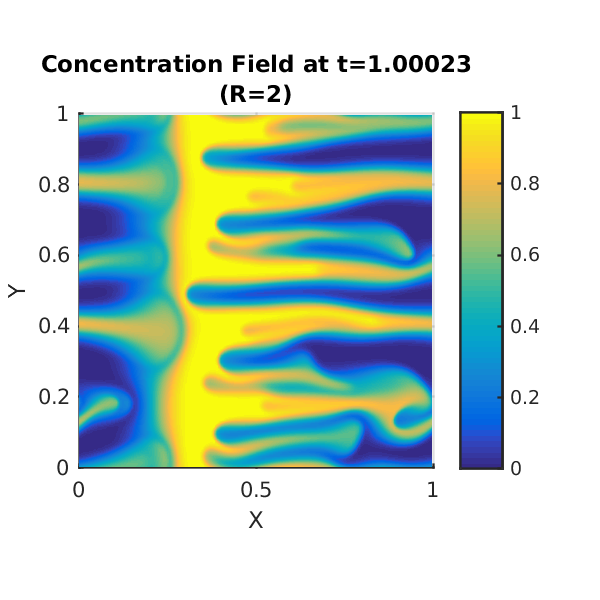
\includegraphics[scale=0.5]{conc20_100.png} &
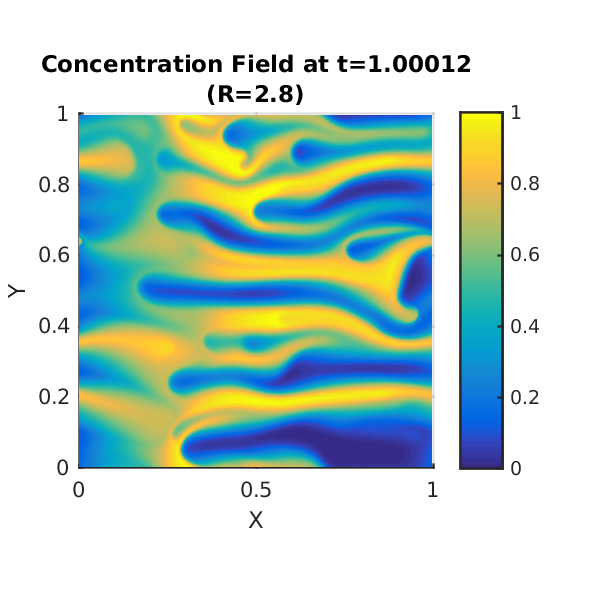
\includegraphics[scale=0.5]{conc28_100.png} \\
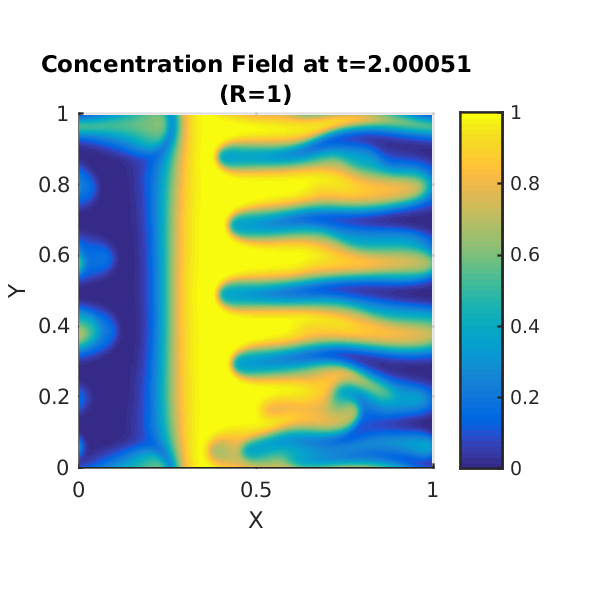
\includegraphics[scale=0.5]{conc10_200.png} &
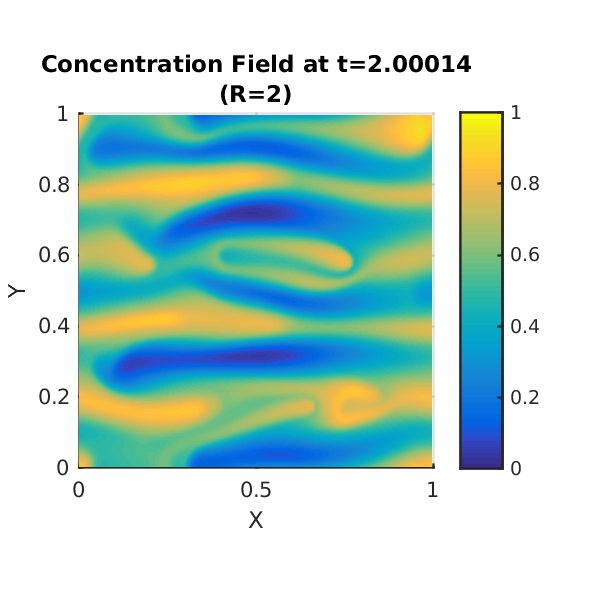
\includegraphics[scale=0.5]{conc20_200.png} &
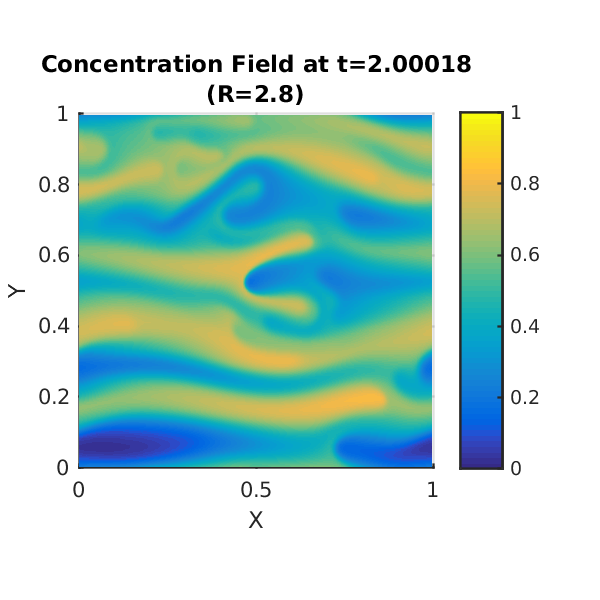
\includegraphics[scale=0.5]{conc28_200.png}
\end{tabular}
\caption{Concentration plots for R = $1, 2, 2.8$ (left to right) at times t $\approx 0.25, 0.5, 1, 2$ (top to bottom).}
\label{fig:conc}
\end{figure}

\clearpage

\begin{figure}[!ht]
\centering
\begin{tabular}{c c c}
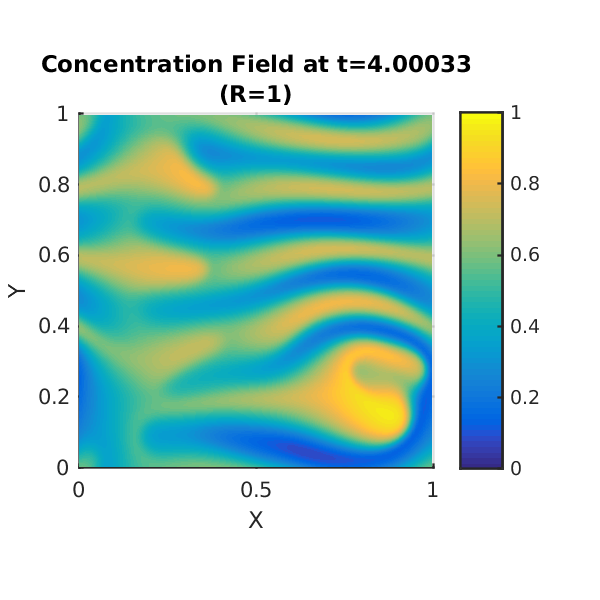
\includegraphics[scale=0.5]{conc10_400.png} &
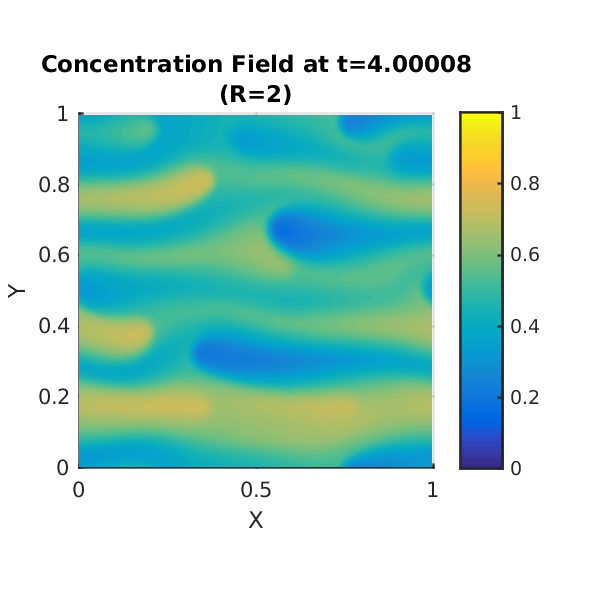
\includegraphics[scale=0.5]{conc20_400.png} &
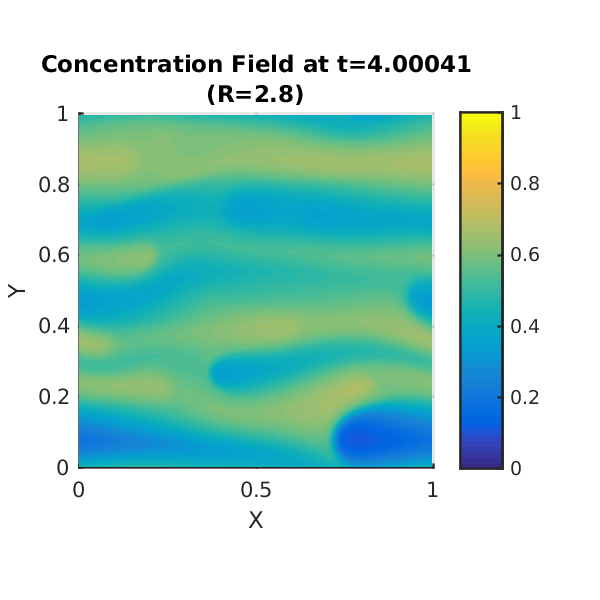
\includegraphics[scale=0.5]{conc28_400.png}
\end{tabular}
\caption{Concentration plots for R = $1, 2, 2.8$ (left to right) at the end of the simulation (t $\approx 4$).}
\label{fig:final-conc}
\end{figure}

\clearpage

\item We have combined the statistics for degree of mixing, mixing rate, and number of fingers into a single figure (figure \ref{fig:concstats}).
From this figure, we notice that the variance in the concentration field goes down linearly with time for the R=1 case (there is a small diffusion-only portion at the very beginning of the simulation).
However, in the R=2 and R=2.8 cases, the function is much sharper and looks nearly exponential (also, the size of the diffusion-only portion at the beginning decreases).
\begin{figure}[!ht]
\centering
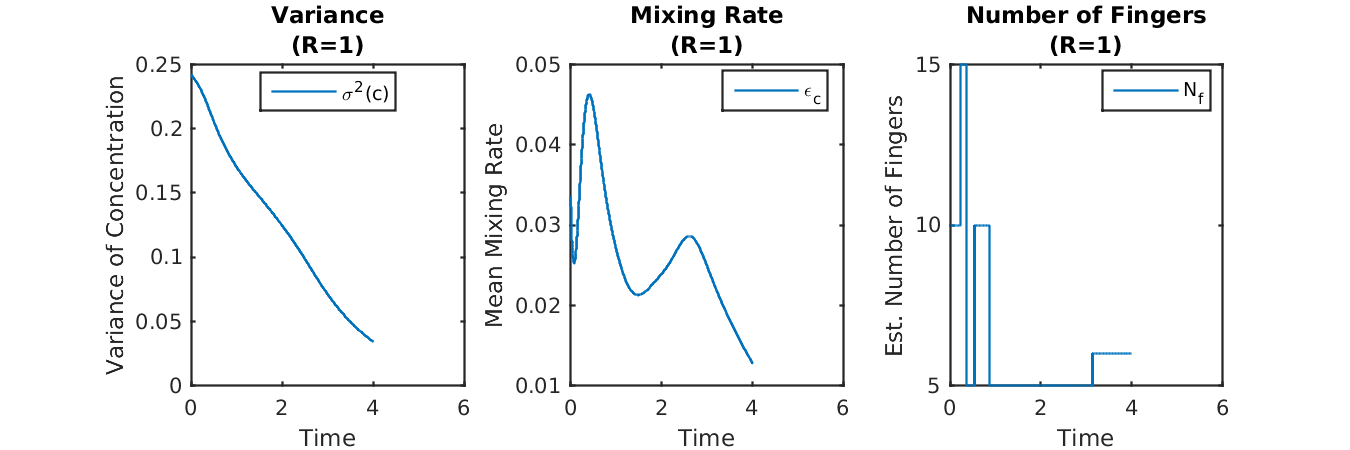
\includegraphics[scale=0.7]{concstats_10.png}
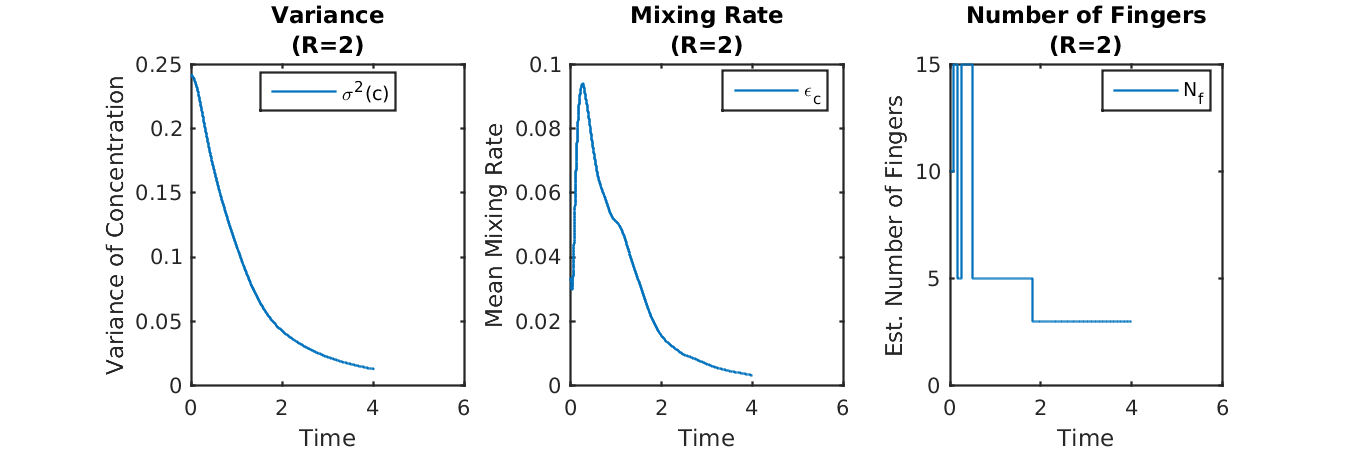
\includegraphics[scale=0.7]{concstats_20.png}
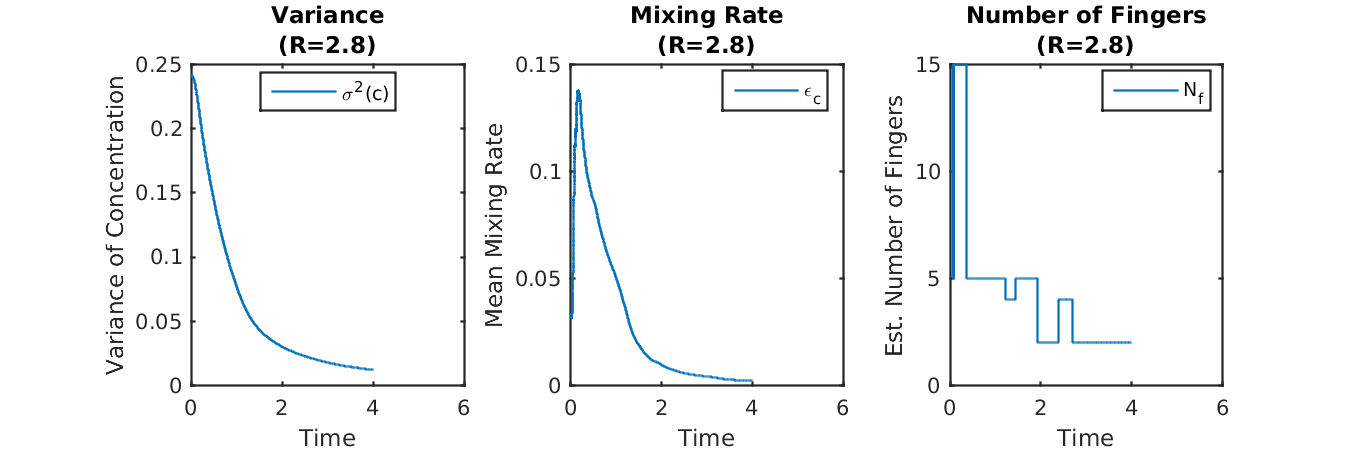
\includegraphics[scale=0.7]{concstats_28.png}
\caption{Evolution of the variance in the concentration field (degree of mixing), $\epsilon_c = (\nabla c \cdot \nabla c) / \mathrm{Pe}$ (rate of mixing), and number of fingers as estimated by the dominant frequency are shown from left to right. Results are given for $R=1, 2, 2.8$ from top to bottom.}
\label{fig:concstats}
\end{figure}

\item For the mixing rate, we notice some special behavior with the R=1 case, which we speculate on in Part 7.
However, otherwise we note that the mixing rate goes up with increasing viscosity contrast and also decays more quickly with increasing viscosity contrast (as a fraction of the maximal value).

\item I am not sure the code to count the fingers is working correctly, but the behavior shown in these plots is at least qualitatively consistent with direct observations from the concentration field.
The initial number of fingers is similar for all the viscosity contrasts due to the seeding.
However, it seems as though the higher viscosity contrast results in more fingers for a short period of time, before they merge into fewer fingers.
As the simulation progresses, more fingers merge until finally the solution is mostly mixed and we have only a few fingers.
In the low contrast case, we continue to see fingers throughout the simulation since the mixing is proceeding slowly.

\end{enumerate}

\subsection{Part 6}
It looks like the main mechanisms for mixing are diffusion and convection through creation of fingers.
Diffusion occurs in the very beginning, but after convection causes fingers to form, gradients are kept sharp and the surface area is increased, leading to more efficient diffusion.
We also have physical transport of the different liquids, but this can lead to channels which are not well-mixed.
Separately, we see certain regions where transient vortex-like structures form, which I imagine enhances mixing (this is more noticeable at high viscosity contrast).

\subsection{Part 7}
It looks like the mixing rate increases with increasing viscosity contrast (look at the scales in figure \ref{fig:concstats}), and similarly the variance in the concentration field shows a sharper decay with increasing viscosity contrast.
However, I know that this trend does not hold, as eventually channels will form and come to dominate (leading to unmixed regions).
I do find it interesting that the variance in concentration is lower at t=2 for R=2.8 than for R=2, while at t=4 they are quite close together.
I suspect if I run it for longer the R=2 case may even go lower than the R=2.8 case, but I did not check this.
Both of these cases are more well-mixed at the end than the R=1 case, which we can confirm visually in the final concentration fields in figure \ref{fig:final-conc}.

Another interesting feature is the increase in mixing rate after about $t \approx 2$ in the $R=1$ case.
This was repeatable, but I am not entirely sure about the mechanism behind it.
I think it's due to fingers merging and reducing mixing rate, but when the (intact) trailing boundary is disturbed by the first fingers, this allows gradients to become larger and lead to increased mixing once again.
Looking at the R=2 case, the trailing boundary is already slightly disturbed by the counterflow fingers, so we don't see a large effect there (a tiny plateau at $t \approx 1$).
With the R=2.8 case, the trailing boundary is severely disturbed by $t \approx 0.75$, so we can't even detect the effect on the mixing rate plot.


\subsection{Part 8}
Since our method is using the spectral method for spatial derivatives, the order is very high (dependent on the total number of grid points).
However, because we use a Runge-Kutta 4 explicit scheme for time integration, we are limited to fourth order accuracy in time.
The RK4 scheme has an interesting convergence region (and is slightly larger than the forward Euler scheme), but it is not the entire left half-plane as in Crank-Nicholson.

Setting the viscosity contrast to a large number is probably not good for the current scheme used (explicit mobility).
This is because explicit methods tend to become unstable if the solution variables change ``too much'' during a step.
With a higher viscosity contrast, the mobilities can change more dramatically between time steps, unless much smaller steps are taken.
For a large viscosity contrast, we will probably want to change to an implicit mobility step, where the stream function and vorticity are solved in a simultaneous manner.
This will be more expensive (and also means we have to create some sort of jacobian matrix), but should allow for larger viscosity contrasts (though we will still be limited by the RK4 scheme for time integration).

For the time derivative, we can add more stages to the Runga-Kutta scheme (which actually improves the stability properties in addition to the order); the trade off is that more evaluations of spatial derivatives are done per time step.

\clearpage
\appendix
\section{Code}
\lstinputlisting[label=code:solve-vel]{../code/calculate_new_velocity.m}
\lstinputlisting[label=code:solve-vel-opt]{../code/calculate_new_velocity_opt.m}
\lstinputlisting[label=code:solve-conc]{../code/calculate_new_concentration.m}
\lstinputlisting[label=code:solve-conc-opt]{../code/calculate_new_concentration_opt.m}
\lstinputlisting[label=code:drive]{../code/drive.m}

\end{document}
